% -----------------------------*- LaTeX -*------------------------------
\documentclass[UTF8]{report}
% ------------------------------------------------------------------------
% Packages
% ------------------------------------------------------------------------
\usepackage{adjustbox}
\usepackage{algorithm,algorithmicx}
\usepackage[noend]{algpseudocode}
\usepackage{amsmath,amsfonts,amssymb,bm,amsthm} % 数学宏包、数学字体、数学符号、支持 \mathscr{} 字体、支持粗斜体 \bm{}、数学定理
\usepackage{bigstrut,multirow,rotating} % Excel表格自动导入latex
\usepackage{booktabs}
\usepackage{breqn}
\usepackage{caption}
\usepackage{color} % 支持颜色改变
\usepackage{ctex}
\usepackage{enumitem} % 自定义列表环境
\usepackage{esint} % 支持多种积分算子
\usepackage{extarrows} % 任意长度的箭头
\usepackage{fancyhdr}
\usepackage{fontsize}
\usepackage{fontspec}
\usepackage[body={7in, 9in},left=1in,right=1in]{geometry}
\usepackage{graphicx} % 支持 \includegraphics{} 插图
\usepackage{mathrsfs}
\usepackage{mathtools} % 数学宏包的重要补充
\usepackage[framemethod=TikZ]{mdframed}
\usepackage{nicefrac}
\usepackage{scribe}
\usepackage{subfigure} % 插入子图
\usepackage{tikz,xcolor} % 画图、画 Feynman 图
\usepackage{upgreek} % 数学环境的直立希腊字母
% ------------------------------------------------------------------------
% Macros
% ------------------------------------------------------------------------
%~~~~~~~~~~~~~~~
% Utility latin
%~~~~~~~~~~~~~~~
\newcommand{\ie}{\textit{i.e.}}
\newcommand{\eg}{\textit{e.g.}}
%~~~~~~~~~~~~~~~
% Environment shortcuts
%~~~~~~~~~~~~~~~
\newcommand{\balign}[1]{\ealign{\begin{align}#1\end{align}}}
\newcommand{\baligns}[1]{\ealigns{\begin{align*}#1\end{align*}}}
\newcommand{\bitemize}[1]{\eitemize{\begin{itemize}#1\end{itemize}}}
\newcommand{\benumerate}[1]{\eenumerate{\begin{enumerate}#1\end{enumerate}}}
%~~~~~~~~~~~~~~~
% Text with quads around it
%~~~~~~~~~~~~~~~
\newcommand{\qtext}[1]{\quad\text{#1}\quad}
%~~~~~~~~~~~~~~~
% Shorthand for math formatting
%~~~~~~~~~~~~~~~
\newcommand{\mbb}[1]{\mathbb{#1}}
\newcommand{\mbi}[1]{\boldsymbol{#1}} % Bold and italic (math bold italic)
\newcommand{\mbf}[1]{\mathbf{#1}}
\newcommand{\mc}[1]{\mathcal{#1}}
\newcommand{\mrm}[1]{\mathrm{#1}}
\newcommand{\tbf}[1]{\textbf{#1}}
\newcommand{\tsc}[1]{\textsc{#1}}
%\def\<{{\langle}}
%\def\>{{\rangle}}
\newcommand{\sT}{\sf T}
\newcommand{\grad}{\nabla}
\newcommand{\Proj}{\Pi}
%~~~~~~~~~~~~~~~
% Common sets 定义数集符号
%~~~~~~~~~~~~~~~
\newcommand{\R}{\mathbb{R}}
\newcommand{\Z}{\mathbb{Z}}
\newcommand{\Q}{\mathbb{Q}}
\newcommand{\N}{\mathbb{N}}
\newcommand{\C}{\mathbb{C}}
\newcommand{\reals}{\mathbb{R}} % Real number symbol
\newcommand{\integers}{\mathbb{Z}} % Integer symbol
\newcommand{\rationals}{\mathbb{Q}} % Rational numbers
\newcommand{\naturals}{\mathbb{N}} % Natural numbers
\newcommand{\complex}{\mathbb{C}} % Complex numbers
%~~~~~~~~~~~~~~~
% Common functions
%~~~~~~~~~~~~~~~
\renewcommand{\exp}[1]{\operatorname{exp}\left(#1\right)} % Exponential
\newcommand{\indic}[1]{\mbb{I}\left(#1\right)} % Indicator function
\newcommand{\indicsub}[2]{\mbb{I}_{#2}\left(#1\right)} % Indicator function
\newcommand{\argmax}{\mathop\mathrm{arg\, max}} % Defining math symbols
\newcommand{\argmin}{\mathop\mathrm{arg\, min}}
\renewcommand{\arccos}{\mathop\mathrm{arccos}}
\newcommand{\dom}{\mathop\mathrm{dom}} % Domain
\newcommand{\range}{\mathop\mathrm{range}} % Range
\newcommand{\diag}{\mathop\mathrm{diag}}
\newcommand{\tr}{\mathop\mathrm{tr}}
\newcommand{\abs}{\mathop\mathrm{abs}}
\newcommand{\card}{\mathop\mathrm{card}}
\newcommand{\sign}{\mathop\mathrm{sign}}
\newcommand{\prox}{\mathrm{prox}} % prox
\newcommand{\rank}[1]{\mathrm{rank}(#1)}
\newcommand{\supp}[1]{\mathrm{supp}(#1)}
\newcommand{\norm}[1]{\lVert#1\rVert}
%~~~~~~~~~~~~~~~
% Common probability symbols
%~~~~~~~~~~~~~~~
\newcommand{\family}{\mathcal{P}} % probability family / statistical model
\newcommand{\iid}{\stackrel{\mathrm{iid}}{\sim}}
\newcommand{\ind}{\stackrel{\mathrm{ind}}{\sim}}
\newcommand{\E}{\mathbb{E}} % Expectation symbol
\newcommand{\Earg}[1]{\E\left[#1\right]}
\newcommand{\Esubarg}[2]{\E_{#1}\left[#2\right]}
\renewcommand{\P}{\mathbb{P}} % Probability symbol
\newcommand{\Parg}[1]{\P\left(#1\right)}
\newcommand{\Psubarg}[2]{\P_{#1}\left[#2\right]}
% \newcommand{\Cov}{\mrm{Cov}} % Covariance symbol
% \newcommand{\Covarg}[1]{\Cov\left[#1\right]}
% \newcommand{\Covsubarg}[2]{\Cov_{#1}\left[#2\right]}
% \newcommand{\model}{\mathcal{P}} % probability family / statistical model
%~~~~~~~~~~~~~~~
% Distributions
%~~~~~~~~~~~~~~~
% \newcommand{\Gsn}{\mathcal{N}}
% \newcommand{\Ber}{\textnormal{Ber}}
% \newcommand{\Bin}{\textnormal{Bin}}
% \newcommand{\Unif}{\textnormal{Unif}}
% \newcommand{\Mult}{\textnormal{Mult}}
% \newcommand{\NegMult}{\textnormal{NegMult}}
% \newcommand{\Dir}{\textnormal{Dir}}
% \newcommand{\Bet}{\textnormal{Beta}}
% \newcommand{\Gam}{\textnormal{Gamma}}
% \newcommand{\Poi}{\textnormal{Poi}}
% \newcommand{\HypGeo}{\textnormal{HypGeo}}
% \newcommand{\GEM}{\textnormal{GEM}}
% \newcommand{\BP}{\textnormal{BP}}
% \newcommand{\DP}{\textnormal{DP}}
% \newcommand{\BeP}{\textnormal{BeP}}
% \newcommand{\Exp}{\textnormal{Exp}}
%~~~~~~~~~~~~~~~
% Theorem-like environments
%~~~~~~~~~~~~~~~
%\theoremstyle{definition}
%\newtheorem{definition}{Definition}
%\newtheorem{example}{Example}
%\newtheorem{problem}{Problem}
%\newtheorem{lemma}{Lemma}
%~~~~~~~~~~~~~~~
% 组合数学的模板和作业里用到的一些宏包和自定义命令
%~~~~~~~~~~~~~~~
\renewcommand{\emph}[1]{\begin{kaishu}#1\end{kaishu}}
\newcommand{\falfac}[1]{^{\underline{#1}}}
\newcommand{\binomfrac}[2]{\frac{#1^{\underline{#2}}}{#2!}}
\newcommand{\ceil}[1]{\left\lceil #1 \right\rceil}
\newcommand{\floor}[1]{\left\lfloor #1 \right\rfloor}
\newcommand{\suminfty}[2]{\sum_{#1=#2}^{\infty}}
\newcommand{\suminftyk}[0]{\sum_{k=0}^{\infty}}
\newcommand{\sumint}[3]{\sum_{#1=#2}^{#3}}
\newcommand{\sumintk}[2]{\sum_{k=#1}^{#2}}
\newcommand{\suminti}[2]{\sum_{i=#1}^{#2}}
%~~~~~~~~~~~~~~~
% 定义新命令
%~~~~~~~~~~~~~~~
\newcommand*{\unit}[1]{\mathop{}\!\mathrm{#1}}
\newcommand*{\dif}{\mathop{}\!\mathrm{d}}%微分算子 d
\newcommand*{\pdif}{\mathop{}\!\partial}%偏微分算子
\newcommand*{\cdif}{\mathop{}\!\nabla}%协变导数、nabla 算子
\newcommand*{\laplace}{\mathop{}\!\Delta}%laplace 算子
\newcommand*{\deriv}[2]{\frac{\mathrm{d} #1}{\mathrm{d} {#2}}}
\newcommand*{\derivh}[3]{\frac{\mathrm{d}^{#1} #2}{\mathrm{d} {#3^{#1}}}}
\newcommand*{\pderiv}[2]{\frac{\partial #1}{\partial {#2}}}
\newcommand*{\pderivh}[3]{\frac{\partial^{#1} #2}{\partial {#3^{#1}}}}
\newcommand*{\dderiv}[2]{\dfrac{\mathrm{d} #1}{\mathrm{d} {#2}}}
\newcommand*{\dderivh}[3]{\dfrac{\mathrm{d}^{#1} #2}{\mathrm{d} {#3^{#1}}}}
\newcommand*{\dpderiv}[2]{\dfrac{\partial #1}{\partial {#2}}}
\newcommand*{\dpderivh}[3]{\dfrac{\partial^{#1} #2}{\partial {#3^{#1}}}}
\newcommand{\me}[1]{\mathrm{e}^{#1}}%e 指数
\newcommand{\mi}{\mathrm{i}}%虚数单位
%\newcommand{\mc}{\mathrm{c}}%光速 定义与mathcal冲突
\newcommand{\red}[1]{\textcolor{red}{#1}}
\newcommand{\blue}[1]{\textcolor{blue}{#1}}
%\newcommand{\Rome}[1]{\setcounter{rome}{#1}\Roman{rome}}
%~~~~~~~~~~~~~~~
% 公式环境中箭头符号的简写
%~~~~~~~~~~~~~~~
\newcommand{\ra}{\rightarrow}
\newcommand{\Ra}{\Rightarrow}
\newcommand{\la}{\leftarrow}
\newcommand{\La}{\Leftarrow}
\newcommand{\lra}{\leftrightarrow}
\newcommand{\Lra}{\Leftrightarrow}
\newcommand{\lgla}{\longleftarrow}
\newcommand{\Lgla}{\Longleftarrow}
\newcommand{\lgra}{\longrightarrow}
\newcommand{\Lgra}{\Longrightarrow}
\newcommand{\lglra}{\longleftrightarrow}
\newcommand{\Lglra}{\Longleftrightarrow}
%~~~~~~~~~~~~~~~
% 一些数学的环境设置
%~~~~~~~~~~~~~~~
%\newcounter{counter_exm}\setcounter{counter_exm}{1}
%\newcounter{counter_prb}\setcounter{counter_prb}{1}
%\newcounter{counter_thm}\setcounter{counter_thm}{1}
%\newcounter{counter_lma}\setcounter{counter_lma}{1}
%\newcounter{counter_dft}\setcounter{counter_dft}{1}
%\newcounter{counter_clm}\setcounter{counter_clm}{1}
%\newcounter{counter_cly}\setcounter{counter_cly}{1}
%\newtheorem{theorem}{{\hskip 1.7em \bf 定理}}
%\newtheorem{lemma}[theorem]{\hskip 1.7em 引理}
%\newtheorem{proposition}[theorem]{Proposition}
%\newtheorem{claim}[theorem]{\hskip 1.7em 命题}
%\newtheorem{corollary}[theorem]{\hskip 1.7em 推论}
%\newtheorem{definition}[theorem]{\hskip 1.7em 定义}
\newcommand{\problem}[1]{{\setlength{\parskip}{10pt}\noindent \bf{#1}}}
\newenvironment{solution}{{\noindent\hskip 2em \bf 解 \quad}}{}
\renewenvironment{proof}{{\setlength{\parskip}{7pt}\noindent\hskip 2em \bf 证明 \quad}}{\hfill$\qed$\par}
%\newenvironment{example}{{\noindent\hskip 2em \bf 例 \arabic{counter_exm}\quad}}{\addtocounter{counter_exm}{1}\par}
%\newenvironment{concept}[1]{{\bf #1\quad} \begin{kaishu}} {\end{kaishu}\par}
%~~~~~~~~~~~~~~~
% 本.tex文档中特殊定义命令
%~~~~~~~~~~~~~~~
\newcommand{\cdclass}[2]{[#1]_{\text{#2}}}
\renewcommand{\to}{$\rightarrow$}

% ----------------------------------------------------------------------
% Header information
% ------------------------------------------------------------------------

\begin{document}

\course{B0911006Y-01} 			%optional
\coursetitle{Computer Organization and Design}	%optional
\semester{2023 Spring}		%optional
\lecturer{Ke Zhang}	%optional
\scribe{吉骏雄}		%required
\lecturenumber{9}			%required (must be a number)
\lecturedate{May 25}	%required (omit year)

\maketitle

% ----------------------------------------------------------------------
% Body of the document
% ------------------------------------------------------------------------


\textbf{9.1,9.3,9.6,9.12,9.14}

\problem{9.1} 设CPU内有这些部件:PC、IR、MAR、MDR、AC、CU。
\begin{enumerate}[label=(\arabic*)]
    \item 写出取指周期的全部微操作。
    \item 写出减法指令``SUB X''、取数指令``LDA X''、存数指令``STA X'' (X 均为主存地址) 在执行阶段所需的全部微操作。
    \item 当上述指令为间接寻址时,写出执行这些指令所需的全部微操作。
    \item 写出无条件转移指令``JMP Y'' 和结果溢出则转指令``BAO Y'' 在执行阶段所需的全部微操作。
\end{enumerate}

\begin{solution}
    \begin{enumerate}[label=(\arabic*)]
        \item
        \begin{itemize}
            \item PC \to MAR
            \item 1 \to R
            \item M(MAR) \to MDR
            \item MDR \to IR
            \item op(IR) \to CU
            \item PC + 1 \to PC
        \end{itemize}

        \item SUB X:
        \begin{itemize}
            \item addr(IR) \to MAR
            \item 1 \to R
            \item M(MAR) \to MDR
            \item AC - MDR \to AC
        \end{itemize}
        LDA X:
        \begin{itemize}
            \item addr(IR) \to MAR
            \item 1 \to R
            \item M(MAR) \to MDR
            \item MDR \to AC
        \end{itemize}
        STA X:
        \begin{itemize}
            \item addr(IR) \to MAR
            \item 1 \to W
            \item AC \to MDR
            \item MDR \to M(MAR)
        \end{itemize}

        \item 如果是间址, 那么它们在非间址阶段的微操作是完全一致的. 在间址阶段, 需要额外的微操作:
        \begin{itemize}
            \item addr(IR) \to MAR
            \item 1 \to R
            \item M(MAR) \to MDR
        \end{itemize}

        \item JMP Y:
        \begin{itemize}
            \item addr(IR) \to PC
        \end{itemize}
        BAO Y:
        \begin{itemize}
            \item O $\cdot$ addr(IR) \to PC
        \end{itemize}

    \end{enumerate}
\end{solution}


\problem{9.3} 什么是指令周期、机器周期和时钟周期?三者有何关系?

\begin{solution}
    指令周期是CPU每取出并执行一条指令执行所需要的全部时间.
    
    机器周期是在同步控制的机器中, CPU执行指令周期中一个步骤所需的时间.
    
    时钟周期是CPU时钟的周期.
    
    通常情况下 (机器周期需要取同样的时钟周期长度), 三者的关系是层层包含的. 一个指令周期由若干个机器周期组成, 一个机器周期由若干个时钟周期组成.
    \[
        \text{指令周期} = \sum \text{机器周期} = \sum\left(\sum\text{指令周期}\right)
    \]
\end{solution}


\problem{9.6} 设某计算机的CPU主频为8MHz ,每个机器周期平均含2个时钟周期,每条指令平均有4个机器周期,试问该计算机的平均指令执行速度为多少MIPS。若CPU主频不变,但每个机器周期平均含4个时钟周期,每条指令平均有4个机器周期,则该机的平均指令执行速度又是多少MIPS? 由此可得出什么结论?

\begin{solution}
    每条指令的时钟周期数为$2 \times 4 = 8 $, 每条指令的执行时间为$8 / 8 \unit{MHZ} = 1 \unit{\mu s}$, 所以该计算机的平均指令执行速度为$1 / 1 \unit{\mu s} = 1MIPS$.

    每条指令的时钟周期数为$4 \times 4 = 16$, 每条指令的执行时间为$16/ 8 \unit{MHZ} = 2 \unit{\mu s}$, 所以该计算机的平均指令执行速度为$1 / 2 \unit{\mu s} = 0.5MIPS$.

    指令执行速度和每个指令周期平均含的时钟周期数成反比, 进而和每个机器周期平均含的时钟周期数成反比.
\end{solution}


\problem{9.12} CPU结构如图,另有B、C、D、E、H、L六个寄存器,写出完成下列指令所需的全部微操作和控制信号(包括取指令)。
\begin{enumerate}[label=(\arabic*)]
    \item 寄存器间接寻址的无条件转移指令``JMP \@ B''。
    \item 间接寻址的存数指令``STA \@ X''。
\end{enumerate}
\begin{figure}[!htbp]
    \centering
    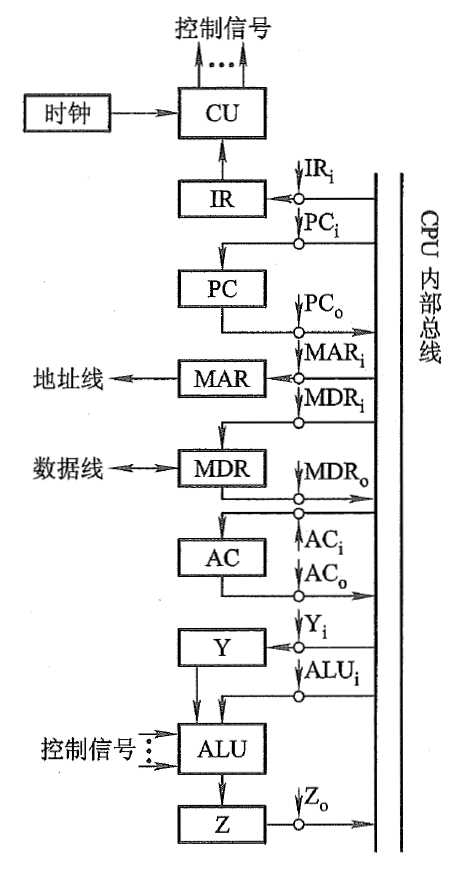
\includegraphics[width=3cm]{fig/9.12.png}
    \caption{9.12题图}
    \label{fig:9_12}
\end{figure}

\newpage

\begin{solution}
    \begin{enumerate}[label=(\arabic*)]
        \item JMP \@ B:
        \begin{table}[htbp]
            \centering
            \begin{tabular}{cl}
                \toprule
                微操作 & 控制信号 \\
                \midrule
                PC \to Bus \to MAR        & $\mathrm{PC_o, MAR_i                   }$\\
                M(MAR) \to MDR            & $\mathrm{MAR_o, MDR_i, R/\overline{W}  }$\\
                MDR \to Bus \to IR        & $\mathrm{MDR_o, IR_i                   }$\\
                PC + 1 \to PC             & $\mathrm{+1                            }$\\
                \midrule
                B \to MAR                 & $\mathrm{B_o, MAR_i                    }$\\
                M(MAR) \to MDR            & $\mathrm{MAR_o, MDR_i, R/\overline{W}  }$\\
                addr(MDR) \to Bus \to PC  & $\mathrm{MDR_o, PC_i                   }$\\
                \bottomrule
            \end{tabular}
        \end{table}

        \newpage

        \item STA \@ X。
        \begin{table}[htbp]
            \centering
            \begin{tabular}{cl}
                \toprule
                微操作 & 控制信号 \\
                \midrule
                PC \to Bus \to MAR        & $\mathrm{PC_o, MAR_i                   }$\\
                M(MAR) \to MDR            & $\mathrm{MAR_o, MDR_i, R/\overline{W}  }$\\
                MDR \to Bus \to IR        & $\mathrm{MDR_o, IR_i                   }$\\
                PC + 1 \to PC             & $\mathrm{+1                            }$\\
                \midrule
                X \to MAR                 & $\mathrm{X_o, MAR_i                    }$\\
                M(MAR) \to MDR            & $\mathrm{MAR_o, MDR_i, R/\overline{W}  }$\\
                MDR \to Bus \to MAR       & $\mathrm{MDR_o, MAR_i                  }$\\
                AC \to Bus \to MDR        & $\mathrm{AC_o, MDR_i                   }$\\
                MDR \to Bus \to M(MAR)    & $\mathrm{MDR_o, MAR_o, W/\overline{R}  }$\\
                \bottomrule
            \end{tabular}
        \end{table}
    \end{enumerate}
\end{solution}


\problem{9.14} 设单总线计算机结构如图9.5所示,其中M 为主存, XR 为变址寄存器, EAR 为有效地址寄存器,LATCH 为锁存器。假设指令地址已存于PC 中,画出``LDA * D'' 和``SUB X,D'' 指令周期信息流程图,并列出相应的控制信号序列。
说明:
\begin{enumerate}[label=(\arabic*)]
    \item ``LDA * D'' 指令字中*表示相对寻址, D 为相对位移量。
    \item ``SUB X,D'' 指令字中X为变址寄存器XR, D 为形式地址。
    \item 寄存器的输入和输出均受控制信号控制,例如, $\mathrm{PC_i}$ 表示PC的输入控制信号, $\mathrm{MDR_o}$表示MDR的输出控制信号。
    \item 凡是需要经过总线实现寄存器之间的传送,需在流程图中注明,如$\mathrm{PC \rightarrow Bus \rightarrow MAR}$,相应的控制信号为$\mathrm{PC_o}$和$\mathrm{MAR_i}$
\end{enumerate}
\begin{figure}[!htbp]
    \centering
    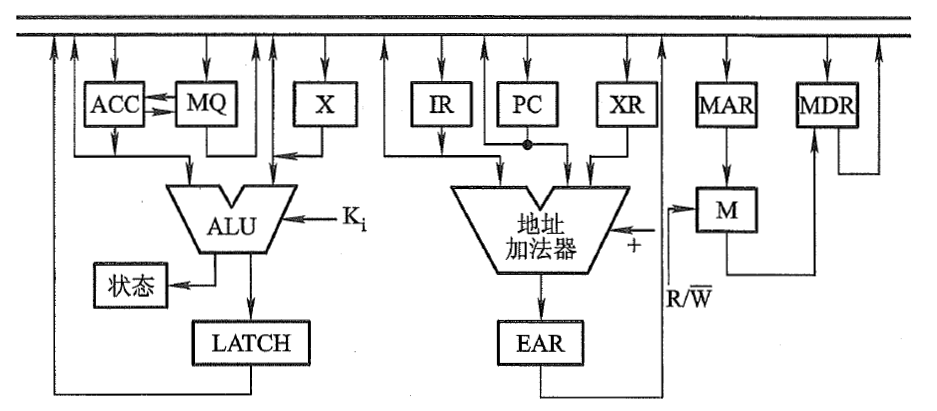
\includegraphics[width=9cm]{fig/9.14.png}
    \caption{9.14题图}
    \label{fig:9_14}
\end{figure}

\newpage

\begin{solution}
        LDA * D:
        \begin{table}[htbp]
            \centering
            \begin{tabular}{cl}
                \toprule
                微操作 & 控制信号 \\
                \midrule
                PC \to Bus \to MAR        & $\mathrm{PC_o, MAR_i                   }$ \\
                M(MAR) \to MDR            & $\mathrm{MAR_o, MDR_i, R/\overline{W}  }$ \\
                MDR \to Bus \to IR        & $\mathrm{MDR_o, IR_i                   }$ \\
                PC + 1 \to PC             & $\mathrm{+1                            }$ \\
                \midrule
                PC + addr(IR) \to EAR     & $\mathrm{PC_o, IR_o, +, EAR_i          }$ \\
                EAR \to Bus \to MAR       & $\mathrm{EAR_o, MAR_i                  }$ \\
                M(MAR) \to MDR            & $\mathrm{MAR_o, MDR_i, R/\overline{W}  }$ \\
                MDR \to Bus \to ACC       & $\mathrm{MDR_o, ACC_i                  }$ \\
                \bottomrule
            \end{tabular}
        \end{table}
        
        SUB X,D:
        \begin{table}[htbp]
            \centering
            \begin{tabular}{cl}
                \toprule
                微操作 & 控制信号 \\
                \midrule
                PC \to Bus \to MAR        & $\mathrm{PC_o, MAR_i                   }$ \\
                M(MAR) \to MDR            & $\mathrm{MAR_o, MDR_i, R/\overline{W}  }$ \\
                MDR \to Bus \to IR        & $\mathrm{MDR_o, IR_i                   }$ \\
                PC + 1 \to PC             & $\mathrm{+1                            }$ \\
                \midrule
                XR + addr(IR) \to EAR     & $\mathrm{XR_o, IR_o, +, EAR_i          }$ \\
                EAR \to Bus \to MAR       & $\mathrm{EAR_o, MAR_i                  }$ \\
                M(MAR) \to MDR            & $\mathrm{MAR_o, MDR_i, R/\overline{W}  }$ \\
                MDR \to Bus \to X         & $\mathrm{MDR_o, X_i                    }$ \\
                ACC - X \to LATCH         & $\mathrm{ACC_o, X_o, K_i=-, LATCH_i    }$ \\
                LATCH \to Bus \to ACC     & $\mathrm{LATCH_o, ACC_i                }$ \\
                \bottomrule
            \end{tabular}
        \end{table}
\end{solution}














\end{document}